\let\negmedspace\undefined
\let\negthickspace\undefined
\documentclass[journal]{IEEEtran}
\usepackage[a5paper, margin=10mm, onecolumn]{geometry}
\usepackage{lmodern} % Ensure lmodern is loaded for pdflatex
\usepackage{tfrupee} % Include tfrupee package

\setlength{\headheight}{1cm} % Set the height of the header box
\setlength{\headsep}{0mm}  % Set the distance between the header box and the top of the text

\usepackage{csquotes}
\usepackage{gvv-book}
\usepackage{gvv}
\usepackage{circuitikz}
\usepackage{cite}
\usepackage{amsmath,amssymb,amsfonts,amsthm}
\usepackage{algorithmic}
\usepackage{graphicx}
\usepackage{textcomp}
\usepackage{xcolor}
\usepackage{txfonts}
\usepackage{listings}
\usepackage{enumitem}
\usepackage{mathtools}
\usepackage{gensymb}
\usepackage{comment}
\usepackage[breaklinks=true]{hyperref}
\usepackage{tkz-euclide} 
\usepackage{listings}
% \usepackage{gvv}                                        
\def\inputGnumericTable{}                                 
\usepackage[latin1]{inputenc}                                
\usepackage{color}                                            
\usepackage{array}                                            
\usepackage{longtable}                                       
\usepackage{calc}                                             
\usepackage{multirow}                                         
\usepackage{hhline}                                           
\usepackage{ifthen}                                           
\usepackage{lscape}
\usepackage{caption}
\usepackage{tikz}
\usetikzlibrary{patterns}
\begin{document}

\bibliographystyle{IEEEtran}



\title{GATE 2008 CIVIL ENGINEERING}
\author{EE25BTECH11013 - Bhargav}
\maketitle
% \maketitle
% \newpage
% \bigskip
{\let\newpage\relax\maketitle}

\renewcommand{\thefigure}{\theenumi}
\renewcommand{\thetable}{\theenumi}
\setlength{\intextsep}{10pt} % Space between text and floats


\section*{Q.1 $-$ Q.20 carry one mark each.}

\begin{enumerate}
\item The product of matrices $\brak{PQ}^{-1} P$ is \hfill \brak{GATE \ CE \ 2008}
\begin{enumerate}
\item $P^{-1}$
\item $Q^{-1}$
\item $P^{-1}Q^{-1}P$
\item $PQ^{-1}$
\end{enumerate}


\item The general solution of 
\begin{align} 
\frac{d^2y}{dx^2} + y = 0
\end{align}
is  \hfill \brak{GATE \ CE \ 2008}
\begin{enumerate}
\begin{multicols}{2}
\item $y = P \cos x + Q \sin x$ 
\item $y = P \cos x$ 
\item $y = P \sin x$
\item $y = P \sin^2 x$
\end{multicols}
\end{enumerate}


\item A mild steel specimen is under uni-axial tensile stress. Young's modulus and yield stress for mild steel are $2 \times 10^5$ MPa and $250$ MPa respectively. The maximum amount of strain energy per unit volume that can be stored in this specimen without permanent set is \hfill \brak{GATE \ CE \ 2008}

\begin{enumerate}
\begin{multicols}{2}
\item $156$ Nmm/mm$^3$ 
\item $15.6$ Nmm/mm$^3$ 
\item $1.56$ Nmm/mm$^3$ 
\item $0.156$ Nmm/mm$^3$
\end{multicols}
\end{enumerate}

\item A reinforced concrete structure has to be constructed along a sea coast. The minimum grade of concrete to be used as per IS:456 - 2000 is  \hfill \brak{GATE \ CE \ 2008}
\begin{enumerate}
\begin{multicols}{4}
\item M 15 
\item M 20 
\item M 25 
\item M 30
\end{multicols}
\end{enumerate}

\item In the design of a reinforced concrete beam, the requirement for bond is not getting satisfied. The economical option to satisfy the requirement for bond is by  \hfill \brak{GATE \ CE \ 2008}

\begin{enumerate}
\item bundling of bars 
\item providing smaller diameter bars more in number 
\item  providing larger diameter bars less in number 
\item providing same diameter bars more in number
\end{enumerate}


\item The shape of the cross-section, which has the largest shape factor, is  \hfill \brak{GATE \ CE \ 2008}

\begin{enumerate}
\begin{multicols}{2}

\item rectangular
\item  I-section
\item  diamond
\item solid circular
\end{multicols}
\end{enumerate}




\item  Group symbols assigned to silty sand and clayey sand are respectively  \hfill \brak{GATE \ CE \ 2008}
\begin{enumerate}
\begin{multicols}{4}
\item SS and CS
\item  SM and SC
\item SM and CS
\item MS and CS
\end{multicols}
\end{enumerate}

\item When a retaining wall moves away from the backfill, the pressure exerted on the wall is termed as \hfill \brak{GATE \ CE \ 2008}


\begin{enumerate}
\item passive earth pressure
\item swelling pressure
\item pore pressure
\item active earth pressure
\end{enumerate}


\item 
Compaction by vibratory roller is the best method of compaction in case of  \hfill \brak{GATE \ CE \ 2008}
\begin{enumerate}
\begin{multicols}{2}
\item moist silty sand
\item well graded dry sand
\item clay of medium compressibility
\item silt of high compressibility
\end{multicols}
\end{enumerate}

\item A person standing on the bank of a canal drops a stone on the water surface. He notices that the disturbance on the water surface in not traveling upstream. This is because the flow in the canal is \hfill \brak{GATE \ CE \ 2008}
\begin{enumerate}
\begin{multicols}{2}
\item sub-critical
\item super-critical 
\item steady 
\item uniform
\end{multicols}
\end{enumerate}


\item A flood wave with a known inflow hydrograph is routed through a large reservoir. The outflow hydrograph will have \hfill \brak{GATE \ CE \ 2008}

\begin{enumerate}
\item attenuated peak with reduced time-base 
\item attenuated peak with increased time-base 
\item increased peak with increased time-base 
\item increased peak with reduced time-base

\end{enumerate}


\item A stable channel is to be designed for a discharge of $Q$ m$^{3}$/s with silt factor $f$ as per Lacey's method. The mean flow velocity \brak{m/s} in the channel is obtained by \hfill \brak{GATE \ CE \ 2008}
\begin{enumerate}
\begin{multicols}{2}
\item $(Qf^{2}/140)^{1/6}$ 
\item $(Qf/140)^{1/3}$ 
\item $(Q^{2}f^{2}/140)^{1/6}$ 
\item $0.48(Q/f)^{1/3}$
\end{multicols}
\end{enumerate}

\item The base width of an elementary profile of a gravity dam of height $H$ is $b$. The specific gravity of the material of the dam is $G$ and uplift pressure coefficient is $K$. The correct relationship for no tension at the heel is given by: \hfill \brak{GATE \ CE \ 2008}
\begin{enumerate}
\begin{multicols}{4}
\item $\frac{b}{H} = \frac{1}{\sqrt{G - K}}$ 
\item $\frac{b}{H} = \sqrt{G - K}$
\item $\frac{b}{H} = \frac{1}{G - K}$


\item $\frac{b}{H} = \frac{1}{K \sqrt{G - K}}$
\end{multicols}
\end{enumerate}

\item Two primary air pollutants are: \hfill \brak{GATE \ CE \ 2008}
\begin{enumerate}
\begin{multicols}{2}
\item sulphur oxide and ozone  
\item nitrogen oxide and peroxyacetyl nitrate  
\item sulphur oxide and hydrocarbon  
\item ozone and peroxyacetyl nitrate
\end{multicols}
\end{enumerate}

\item Two biodegradable components of municipal solid waste are: \hfill \brak{GATE \ CE \ 2008}
\begin{enumerate}
\begin{multicols}{2}
\item plastics and wood
\item cardboard and glass
\item leather and tin cans 
\item food wastes and garden trimmings
\end{multicols}
\end{enumerate}

\item The specific gravity of paving bitumen as per IS:$73$ -- $1992$ lies between: \hfill \brak{GATE \ CE \ 2008}
\begin{enumerate}
\begin{multicols}{2}
\item 1.10 and 1.06  
\item 1.06 and 1.02  
\item 1.02 and 0.97  
\item 0.97 and 0.92
\end{multicols}
\end{enumerate}

\item A combined value of flakiness and elongation index is to be determined for a sample of aggregates. The sequence in which the two tests are conducted is: \hfill \brak{GATE \ CE \ 2008}

\begin{enumerate}
\item elongation index test followed by flakiness index test on the whole sample
\item flakiness index test followed by elongation index test on the whole sample
\item flakiness index test followed by elongation index test on non-flaky aggregates
\item elongation index test followed by flakiness index test on non-elongated aggregates
\end{enumerate}

\item The capacities of One-way $1.5 m$ wide sidewalk persons per hour and One-way 2-lane urban road 
{\fontsize{9}{7}\selectfont \brak{PCU \ per \ hour, with \ no \ frontage \ access, \ no \ standing \ vehicles, \ and \ very \ little \ cross \ traffic}}
 are respectively: 
\hfill \brak{GATE \ CE \ 2008}

\begin{enumerate}
\begin{multicols}{2}
\item $1.10$ and $1.06$  
\item $1.06$ and $1.02$  
\item $1.02$ and $0.97$  
\item $0.97$ and $0.92$
\end{multicols}
\end{enumerate}

\item The shape of the STOP sign according to IRC:$67$ -- $2001$ is: \hfill \brak{GATE \ CE \ 2008}
\begin{enumerate}
\begin{multicols}{2}
\item circular 
\item triangular
\item octagonal 
\item rectangular
\end{multicols}
\end{enumerate}

\item The type of surveying in which the curvature of the earth is taken into account is called: \hfill \brak{GATE \ CE \ 2008}
\begin{enumerate}
\begin{multicols}{2}
\item Geodetic surveying 
\item Plane surveying
\item Preliminary surveying 
\item Topographical surveying
\end{multicols}
\end{enumerate}

\section*{Q.21 $-$ Q.75 carry two marks each.}

\item The equation 
\begin{align}
k_x \frac{\partial^2 h}{\partial x^2} + k_z \frac{\partial^2 h}{\partial z^2} = 0
\end{align}
can be transformed to \begin{align}
\frac{\partial^2 h}{\partial x_t^2} + \frac{\partial^2 h}{\partial z^2} = 0
\end{align}
by substituting: \hfill \brak{GATE \ CE \ 2008}
\begin{enumerate}
\begin{multicols}{2}
\item $x_t = x \frac{k_z}{k_x}$
\item $x_t = x \frac{k_x}{k_z}$
\item $x_t = x \sqrt{\frac{k_x}{k_z}}$
\item $x_t = x \sqrt{\frac{k_z}{k_x}}$
\end{multicols}
\end{enumerate}

\item The value of 
\begin{align}
\int_0^3 \int_0^{3-x} (6 - x - y) \, dx \, dy \quad \text{is}
\end{align}
\hfill \brak{GATE \ CE \ 2008}
\begin{enumerate}
\begin{multicols}{2}
\item $13.5$
\item $27.0$
\item $40.5$
\item $54.0$
\end{multicols}
\end{enumerate}

\item Three values of $x$ and $y$ are to be fitted in a straight line in the form $y = a + bx$ by the method of least squares. Given: $\sum x = 6$, $\sum y = 21$, $\sum x^2 = 14$ and $\sum xy = 46$, the values of $a$ and $b$ are respectively: \hfill \brak{GATE \ CE \ 2008}
\begin{enumerate}
\begin{multicols}{2}
\item $2$ and $3$
\item $1$ and $2$
\item $2$ and $1$
\item $3$ and $2$
\end{multicols}
\end{enumerate}

\item Solution of \begin{align} \frac{dy}{dx} = \frac{-x}{y} \end{align}at $x = 1$ and $y = \sqrt{3}$ is: \hfill \brak{GATE \ CE \ 2008}
\begin{enumerate}
\begin{multicols}{2}
\item $x^2 - y^2 = -2$
\item $x^2 + y^2 = 4$
\item $x^2 - y^2 = -2$
\item $x^2 + y^2 = 4$
\end{multicols}
\end{enumerate}

\item If the probability density function of a random variable $X$ is  
\begin{align}
f(x) = 
\begin{cases}
x^2, & \text{for } -1 \leq x \leq 1 \\
0, & \text{for any other value of } x
\end{cases}
\end{align}
then, the percentage probability $P\left( -\frac{1}{3} \leq x \leq \frac{1}{3} \right)$ is: \hfill \brak{GATE \ CE \ 2008}
\begin{enumerate}
\begin{multicols}{2}
\item $0.247$
\item $2.47$
\item $24.7$
\item $247$
\end{multicols}
\end{enumerate}

\item The Eigen values of the matrix \hfill \brak{GATE \ CE \ 2008}
\begin{align}
\mathbf{P} = \myvec{$4$ & $-5$ \\ $2$ & $-5$}
\end{align}
are:
\begin{enumerate}
\begin{multicols}{2}
\item $-7$ and $8$
\item $-6$ and $5$
\item $3$ and $4$
\item $1$ and $2$
\end{multicols}
\end{enumerate}

\item A person on a trip has a choice between private car and public transport. The probability of using a private car is $0.45$. While using the public transport, further choices available are bus and metro, out of which the probability of commuting by a bus is $0.55$. In such a situation, the probability \brak{rounded \  up \  to\  two \  decimals} of using a car, bus and metro, respectively would be: \hfill \brak{GATE \ CE \ 2008}
\begin{enumerate}
\begin{multicols}{2}
\item $0.45$, $0.30$ and $0.25$
\item $0.45$, $0.25$ and $0.30$
\item $0.45$, $0.55$ and $0.00$
\item $0.45$, $0.35$ and $0.20$
\end{multicols}
\end{enumerate}

\item The following simultaneous equations: 

\begin{align}
x + y + z &= 3 \\
x + 2y + 3z &= 4 \\
x + 4y + kz &= 6
\end{align}

will NOT have a unique solution for $k$ equal to: \hfill \brak{GATE \ CE \ 2008}
\begin{enumerate}
\begin{multicols}{2}
\item $0$
\item $5$
\item $6$
\item $7$
\end{multicols}
\end{enumerate}

\item The inner \brak{dot} product of two vectors $\vec{P}$ and $\vec{Q}$ is zero. The angle \brak{degrees} between the two vectors is: \hfill \brak{GATE \ CE \ 2008}
\begin{enumerate}
\begin{multicols}{2}
\item $0$
\item $30$
\item $90$
\item $120$
\end{multicols}
\end{enumerate}

\item Cross-section of a column consisting of two steel strips, each of thickness $t$ and width $b$ is shown in the figure below. The critical loads of the column with perfect bond and without bond between the strips are $P$ and $P_0$ respectively. The ratio $P/P_0$ is: \hfill \brak{GATE \ CE \ 2008}

\begin{figure}[H]
    \centering
    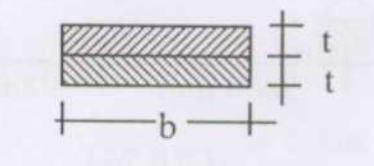
\includegraphics[width=0.3\columnwidth]{figs/fig14.png} 
    \caption{Cross-section of 2 steel strips}
    \label{fig:placeholder}
\end{figure}

\begin{enumerate}
\begin{multicols}{2}
\item $2$
\item $4$
\item $6$
\item $8$
\end{multicols}
\end{enumerate}

\item A rigid bar $GH$ of length $L$ is supported by a hinge and a spring of stiffness $K$ as shown in the figure below. The buckling load, $P_Cr$, for the bar will be  \hfill \brak{GATE \ CE \ 2008}

\begin{figure}[H]
    \centering
    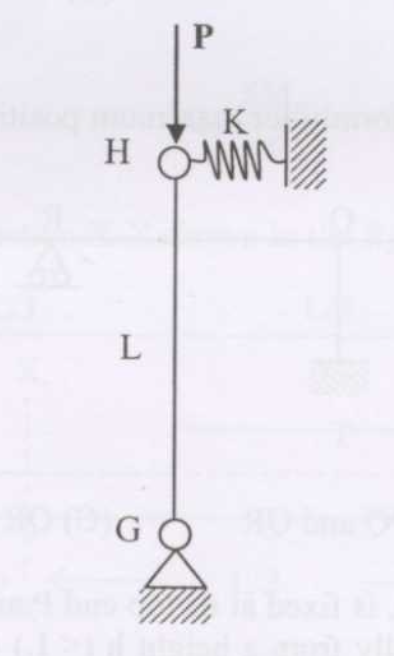
\includegraphics[width=0.2\columnwidth]{figs/fig15.png} 
    \caption{Rigid Bar GH}
    \label{fig:placeholder}
\end{figure}
\begin{enumerate}
\begin{multicols}{2}
\item $0.5 KL$
\item $0.8 KL$
\item $1.0 KL$
\item $1.2 KL$
\end{multicols}
\end{enumerate}



\item The degree of static indeterminacy of the rigid frame having two internal hinges as shown in the figure below, is \hfill \brak{GATE \ CE \ 2008}


\begin{figure}[H]
    \centering
    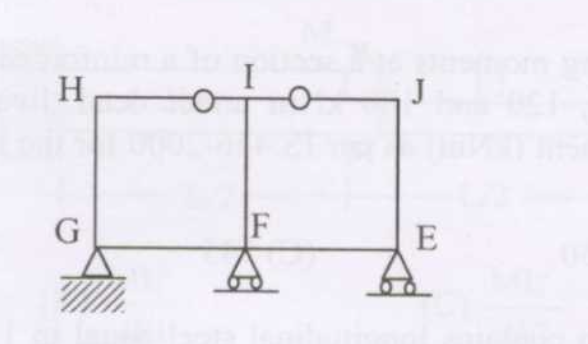
\includegraphics[width=0.6\columnwidth]{figs/fig6.png} 
    \caption{Rigid Frame GHIJEF}
    \label{fig:placeholder}
\end{figure}

\begin{enumerate}
\begin{multicols}{2}
\item $8$
\item $7$
\item $6$
\item $5$
\end{multicols}
\end{enumerate}



\item The members EJ and IJ of a steel truss shown in the figure below are subjected to a temperature rise of $30^\degree\text{C}$. The coefficient of thermal expansion of steel is $0.000012$ per $^\degree\text{C}$ per unit length. The displacement \brak{mm} of joint E relative to joint H along the direction HE of the truss, is \hfill \brak{GATE \ CE \ 2008}
\begin{figure}[H]
    \centering
    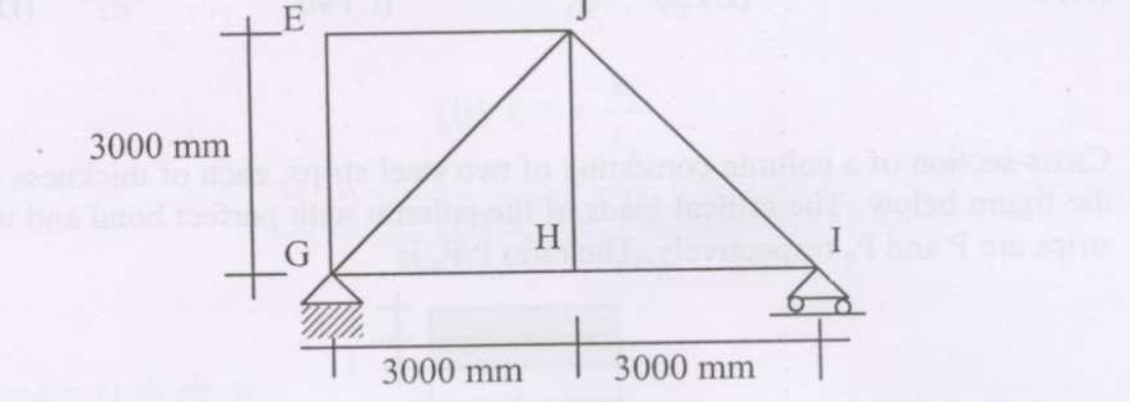
\includegraphics[width=0.6\columnwidth]{figs/fig7.png} 
    \caption{Steel Truss}
    \label{fig:placeholder}
\end{figure}
\begin{enumerate}
\begin{multicols}{2}
\item $0.255$
\item $0.589$
\item $0.764$
\item $1.026$
\end{multicols}
\end{enumerate}

\item The maximum shear stress in a solid shaft of circular cross-section having diameter $d$ subjected to a torque $T$ is $\tau$. If the torque is increased by four times and the diameter of the shaft is increased by two times, the maximum shear stress in the shaft will be  \hfill \brak{GATE \ CE \ 2008}
\begin{enumerate}
\begin{multicols}{2}
\item $2\tau$
\item $\tau$
\item $\tau /2$
\item $\tau /4$
\end{multicols}
\end{enumerate}

\item The span\brak{s} to be loaded uniformly for maximum positive \brak{upward} reaction at support P, as shown in the figure below, is\brak{are} \hfill \brak{GATE \ CE \ 2008}
\begin{figure}[H]
    \centering
    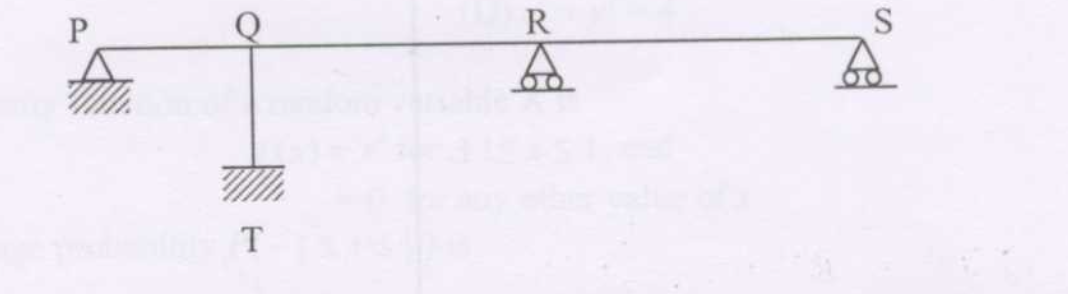
\includegraphics[width=0.6\columnwidth]{figs/fig8.png} 
    \caption{Maximum reaction at P}
    \label{fig:placeholder}
\end{figure}



\begin{enumerate}
\begin{multicols}{2}
\item $PQ$ only
\item $PQ$ and $QR$
\item $QR$ and $RS$
\item $PQ$ and $RS$
\end{multicols}
\end{enumerate}

\item A vertical rod PQ of length L is fixed at its top end P and has a flange fixed to the bottom end Q. A weight $W$ is dropped vertically from a height $h$ < $L$ on to the flange. The axial stress in the rod can be reduced by \hfill \brak{GATE \ CE \ 2008}

\begin{enumerate}
\item increasing the length of the rod 
\item decreasing the length of the rod
\item decreasing the area of cross-section of the rod
\item increasing the modulus of elasticity of the material
\end{enumerate}

\item Un-factored maximum bending moments at a section of a reinforced concrete beam resulting from
a frame analysis are $50$, $80$, $120$ and $180$ kNm under dead, live, wind and earthquake loads
respectively. The design moment \brak{kNm} as per IS:456-2000 for the limit state of collapse \brak{flexure}
is \hfill \brak{GATE \ CE \ 2008}

\begin{enumerate}
\item $195$
\item $250$
\item $345$
\item $372$
\end{enumerate}

\item A reinforced concrete column contains longitudinal steel equal to $1$ percent of net cross-sectional area of the column. Assume modular ratio as $10$. The loads carried \brak{using \ the \ elastic \ theory} by the longitudinal steel and the net area of concrete, are $P_s$, and $P_c$, respectively. The ratio $P_s/P_c$ expressed
as percent is \hfill \brak{GATE \ CE \ 2008}

\begin{enumerate}
\item $0.1$
\item $1$
\item $1.1$
\item $10$
\end{enumerate}

\item A pre-tensioned concrete member of section 200 mm x 250 mm contains tendons of area $500$ $mm^{2}$
at centre of gravity of the section. The prestress in the tendons is $1000$ N/$mm^{2}$. Assuming modular
ratio as $10$, the stress N/$mm^{2}$ in concrete is \hfill \brak{GATE \ CE \ 2008}

\begin{enumerate}
\item $11$
\item $9$
\item $7$
\item $5$
\end{enumerate}

\item Rivets and bolts subjected to both shear stress $\tau_{vf,\ \text{cal}}$ and axial tensile stress ($\sigma_{tf,\ \text{cal}}$) shall be so proportioned that the stresses do not exceed the respective allowable stresses $\tau_{vf}$ and $\sigma_{tf}$ and the value of
\begin{align}
\left( \frac{\tau_{vf,\ \text{cal}}}{\tau_{vf}} + \frac{\sigma_{tf,\ \text{cal}}}{\sigma_{tf}} \right)
\end{align}
does not exceed \hfill \brak{GATE \ CE \ 2008}

\begin{enumerate}
\begin{multicols}{4}

\item $1.0$
\item $1.2$
\item $1.4$
\item $1.8$
\end{multicols}
\end{enumerate}

\item A continuous beam is loaded as shown in the figure below. Assuming a plastic moment capacity equal to $M_p$, the minimum load at which the beam would collapse is \hfill \brak{GATE \ CE \ 2008}

\begin{figure}[H]
    \centering
    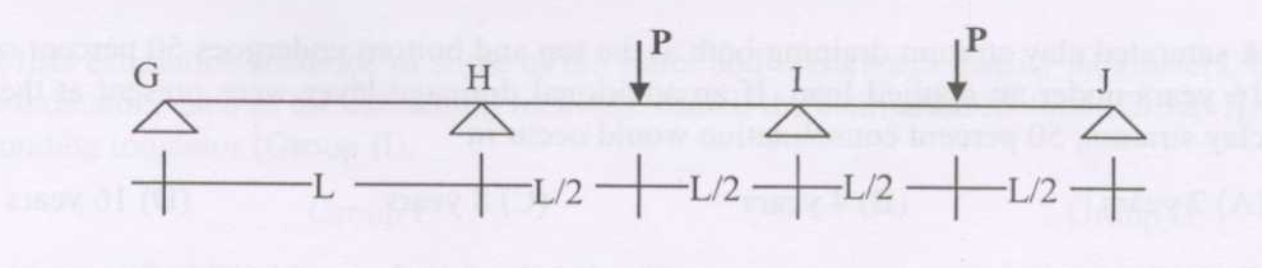
\includegraphics[width=0.6\columnwidth]{figs/fig1.png} 
    \caption{}
    \label{fig:placeholder}
\end{figure} 

\begin{enumerate}
\begin{multicols}{4}
\item $\brak{\frac{4M_p}{L}}$

\item $\brak{\frac{6M_p}{L}}$
\item $\brak{\frac{8M_p}{L}}$

\item $\brak{\frac{10M_p}{L}}$
\end{multicols}
\end{enumerate}

\item The maximum tensile stress at the section X-X shown in the figure below is \hfill \brak{GATE \ CE \ 2008}

\begin{figure}[H]
    \centering
    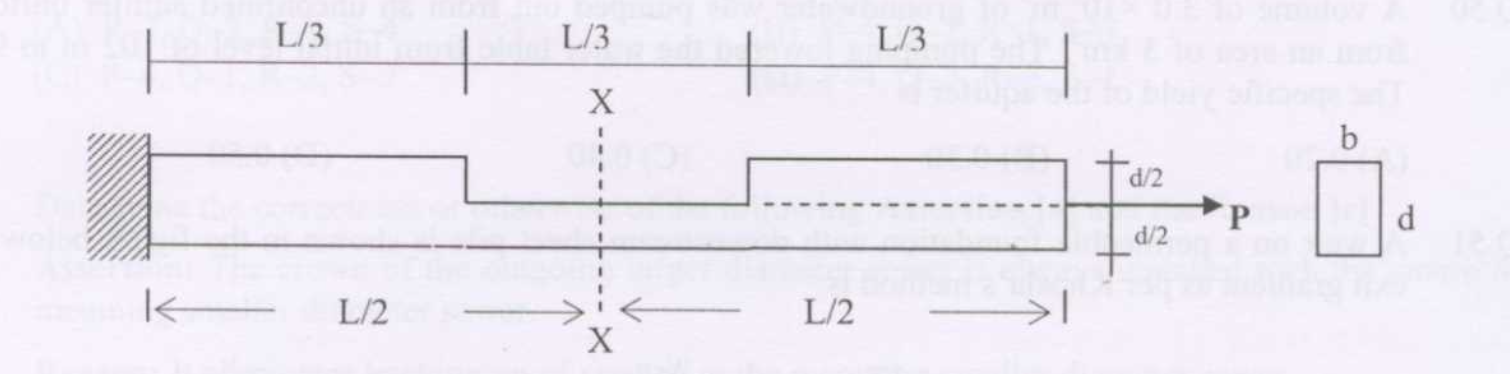
\includegraphics[width=0.6\columnwidth]{figs/fig2.png} 
    \caption{Maximum tensile stress}
    \label{fig:placeholder}
\end{figure}
\begin{enumerate}
\begin{multicols}{4}
\item $\brak{\frac{8P}{bd}}$

\item $\brak{\frac{6P}{bd}}$
\item $\brak{\frac{4P}{bd}}$

\item $\brak{\frac{2P}{bd}}$
\end{multicols}
\end{enumerate}

\item The stepped cantilever is subjected to moments, M as shown in the figure below. The vertical deflection at the free end \brak{neglecting \ the \ self \ weight} is \hfill \brak{GATE \ CE \ 2008}

\begin{figure}[H]
    \centering
    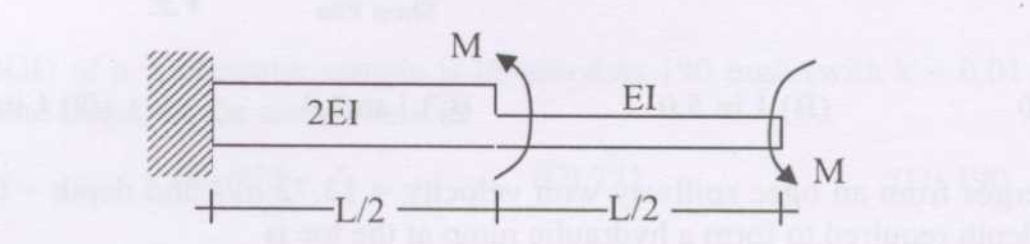
\includegraphics[width=0.6\columnwidth]{figs/fig3.png} 
    \caption{Stepped cantilever}
    \label{fig:placeholder}
\end{figure}
\begin{enumerate}
\begin{multicols}{4}
\item $\brak{\frac{ML^2}{8EI}}$

\item $\brak{\frac{ML^2}{4EI}}$
\item $\brak{\frac{ML^2}{2EI}}$

\item $Zero$
\end{multicols}
\end{enumerate}

\item The liquid limit \brak{LL}, plastic limit \brak{PL} and shrinkage limit \brak{PL} of a cohesive soil satisfy the relation \hfill \brak{GATE \ CE \ 2008}

\begin{enumerate}
\begin{multicols}{2}
\item $LL > PL < SL$

\item $LL > PL > SL$
\item $LL < PL < SL$

\item $LL < PL > SL$
\end{multicols}
\end{enumerate}

\item A footing $2 m \times 1 m$ exerts a uniform pressure of $150$ kN/$m^{2}$ on the soil. Assuming a load
dispersion of 2 vertical to 1 horizontal, the average vertical stress \brak{kN/m} at 1.0 m below the
footing is \hfill \brak{GATE \ CE \ 2008}

\begin{enumerate}
\begin{multicols}{2}
\item $55$
\item $75$
\item $80$
\item $100$
\end{multicols}
\end{enumerate}

\item A direct shear test was conducted on a cohesionless soil \brak{c = 0} specimen under a normal stress of $200$ kN/m?. The specimen failed at a shear stress of $100$ kN/$m^{2}$. The angle of internal friction of the soil \brak{degrees} is \hfill \brak{GATE \ CE \ 2008}

\begin{enumerate}
\begin{multicols}{2}
\item $26.6$
\item $29.5$
\item $30.0$
\item $32.6$
\end{multicols}
\end{enumerate}

\item A pile of $0.50 m$ diameter and of length $10 m$ is embedded in a deposit of clay. The undrained strength parameters of the clay are cohesion = $60 kN/m$ and the angle of internal friction = $0$. The skin friction capacity \brak{kN} of the pile for an adhesion factor of $0.6$, is \hfill \brak{GATE \ CE \ 2008}

\begin{enumerate}
\begin{multicols}{2}
\item $671$
\item $565$
\item $283$
\item $106$
\end{multicols}
\end{enumerate}

\item A saturated clay stratum draining both at the top and bottom undergoes $50$ percent consolidation in $16$ years under an applied load. If an additional drainage layer were present at the middle of the clay stratum, $50$ percent consolidation would occur in \hfill \brak{GATE \ CE \ 2008}

\begin{enumerate}
\begin{multicols}{2}
\item $2$  years
\item $4$  years
\item $8$  years
\item $16$ years
\end{multicols}
\end{enumerate}

\item A test plate $30 cm \times 30 cm$ resting on a sand deposit settles by $10 mm$ under a certain loading intensity. A footing $150 cm \times 200$ cm resting on the same sand deposit and loaded to the same load intensity settles by \hfill \brak{GATE \ CE \ 2008}

\begin{enumerate}
\begin{multicols}{2}
\item $2.0$ mm
\item $27.8$ mm
\item $30.2$ mm
\item $50.0$ mm
\end{multicols}
\end{enumerate}

\item A volume of $3.0 \times 10^{6}$ m of groundwater was pumped out from an unconfined aquifer uniformly from an area of $5$ km. The pumping lowered the water table from initial level of $102$ m to $99$ m. The specific yield of the aquifer is \hfill \brak{GATE \ CE \ 2008}

\begin{enumerate}
\begin{multicols}{2}
\item $0.20$ 
\item $0.30$ 
\item $0.40$ 
\item $0.50$ 
\end{multicols}
\end{enumerate}

\item A weir on a permeable foundation with downstream sheet pile is shown in the figure below. The exit gradient as per Khosla's method is \hfill \brak{GATE \ CE \ 2008}
\begin{figure}[H]
    \centering
    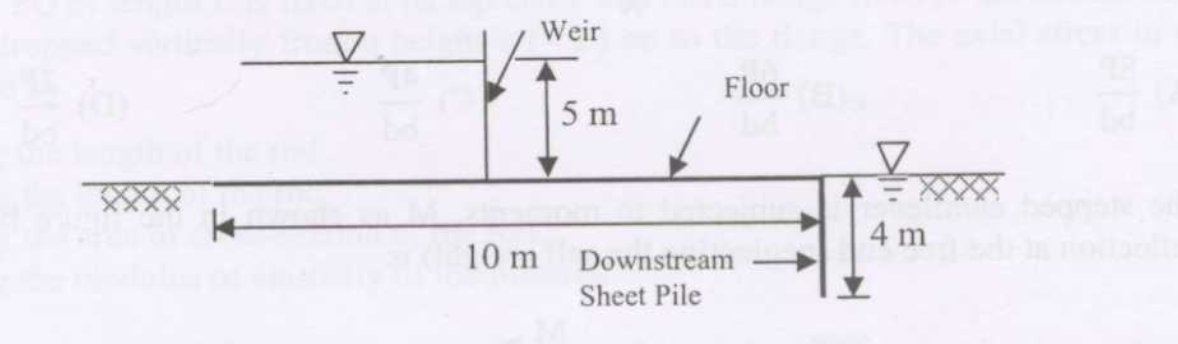
\includegraphics[width=0.6\columnwidth]{figs/fig4.png} 
    \caption{}
    \label{fig:placeholder}
\end{figure}
\begin{enumerate}
\begin{multicols}{2}
\item $1$ in $6.0$ 
\item $1$ in $5.0$ 
\item $1$ in $3.4$ 
\item $1$ in $2.5$ 
\end{multicols}
\end{enumerate}

\item Water emerges from an ogee spillway with velocity = $13.72$ m/s and depth = $0.3$ m at its toe. The tail water depth required to form a hydraulic jump at the toe is \hfill \brak{GATE \ CE \ 2008}

\begin{enumerate}
\begin{multicols}{2}
\item $6.48$ m 
\item $5.24$ m
\item $3.24$ m 
\item $2.24$ m 
\end{multicols}
\end{enumerate}

\item The flow of water (mass density = $1000$ kg/$m^{3}$ and kinematic viscosity = $10^{-6}$ m/s) in a commercial pipe, having equivalent roughness $k_s$, as $0.12$ mm, yields an average shear stress at the pipe boundary = $600$ N/m?. The value of $k_s$/$\delta$ \brak{\delta \ being \ the \ thickness \ of \ laminar \ sub-layer} for this pipe is \hfill \brak{GATE \ CE \ 2008}

\begin{enumerate}
\begin{multicols}{2}
\item $0.25$ m 
\item $0.50$ m
\item $6.0$ m 
\item $8.0$ m 
\end{multicols}
\end{enumerate}

\item A river reach of $2.0$ km long with maximum flood discharge of $10000$ $m^{3}/s$ is to be physically modeled in the laboratory where maximum available discharge is $0.20$ m/s. For a geometrically similar model based on equality of Froude number, the length of the river reach \brak{m} in the model is \hfill \brak{GATE \ CE \ 2008}

\begin{enumerate}
\begin{multicols}{2}
\item $26.4$ m 
\item $25.0$ m
\item $20.5$ m 
\item $18.0$ m 
\end{multicols}
\end{enumerate}

\item An outlet irrigates an area of $20  ha$. The discharge $(l/s)$ required at this outlet to meet the evapo-transpiration requirement of 20 mm occurring uniformly in $20$ days neglecting other field losses is \hfill \brak{GATE \ CE \ 2008}

\begin{enumerate}
\begin{multicols}{2}
\item $2.52$ m 
\item $2.31$ m
\item $2.01$ m 
\item $1.52$ m 
\end{multicols}
\end{enumerate}

\item A wastewater sample contains $10^{-5.6}$ mmol/l of $OH^{-}$ ions at $25$ $^\degree\text{C}$ .The $pH$ of this sample is \hfill \brak{GATE \ CE \ 2008}

\begin{enumerate}
\begin{multicols}{2}
\item $8.6$ 
\item $8.4$
\item $5.6$ 
\item $5.4$ 
\end{multicols}
\end{enumerate}

\item Group $I$ lists estimation methods of some of the water and wastewater quality parameters. Group $II$ lists the indicators used in the estimation methods. Match the estimation method (Group $I$) with the corresponding indicator Group $II$). \hfill \brak{GATE \ CE \ 2008}


\textbf{Group I \hfill Group II}

\begin{tabular}{ll}
P & Azide modified Winkler method for dissolved oxygen \hfill 1. Eriochrome Black T \\
Q & Dichromate method for chemical oxygen demand \hfill 2. Ferrion \\
R & EDTA titrimetric method for hardness \hfill 3. Potassium chromate \\
S & Mohr or Argentometric method for chlorides \hfill 4. Starch \\
\end{tabular}


\textbf{Options:}
\begin{enumerate}
  \item P--3,\quad Q--2,\quad R--1,\quad S--4
  \item P--4,\quad Q--2,\quad R--1,\quad S--3
  \item P--4,\quad Q--1,\quad R--2,\quad S--3
  \item P--4,\quad Q--2,\quad R--3,\quad S--1
\end{enumerate}


\item Determine the correctness or otherwise of the following Assertion [a] and the Reason [r]


Assertion: The crown of the outgoing larger diameter sewer is always matched with the crown of
incoming smaller diameter sewer.


Reason: It eliminates backing up of sewage in the incoming smaller diameter sewer. \hfill \brak{GATE \ CE \ 2008}

\begin{enumerate}
\item Both \sbrak{a} and \sbrak{r} are true and \sbrak{r} is the correct reason for \sbrak{a}
\item Both \sbrak{a} and \sbrak{r} are true but \sbrak{r} is not the correct reason for \sbrak{a}
\item Both \sbrak{a} and \sbrak{r} are false 
\item Assertion \sbrak{a} is true but Reason\sbrak{r} is false 
\end{enumerate}     

\item The $5$-day BOD of a wastewater sample is obtained as $190$ mg/l (with k = $0.01$  $h^{-1}$). The ultimate oxygen demand \brak{mg/l} of the sample will be \hfill \brak{GATE \ CE \ 2008}

\begin{enumerate}
\item $3800$
\item $475$
\item $271$
\item $190$
\end{enumerate}  

\item A water treatment plant is required to process $28800$ $m^{3}$/d of raw water (density = 1000 kg/$m^{3}$, kinematic viscosity = $10$ ms). The rapid mixing tank imparts a velocity gradient of $900$ $s^{-1}$ to blend $35$ mg/l of alum with the flow for a detention time of $2$ minutes. The power input \brak{W} required for rapid mixing is \hfill \brak{GATE \ CE \ 2008}

\begin{enumerate}
\item $32.4$
\item $36$
\item $324$
\item $32400$
\end{enumerate}  

\item Match Group I \brak{Terminology} with Group II \brak{Definition/Brief Description} for wastewater treatment systems \hfill \brak{GATE \ CE \ 2008}

\begin{minipage}[t]{0.45\textwidth}
\textbf{Group I}
\begin{enumerate}[align=left]
    \item[P.] Primary treatment
    \item[Q.] Secondary treatment
    \item[R.] Unit operation
    \item[S.] Unit process
\end{enumerate}
\end{minipage}
\hfill
\begin{minipage}[t]{0.45\textwidth}
\textbf{Group II}
\begin{enumerate}[align=left]
    \item[1.] Contaminant removal by physical forces
    \item[2.] Involving biological and/or chemical reaction
    \item[3.] Conversion of soluble organic matter to biomass
    \item[4.] Removal of solid materials from incoming wastewater
\end{enumerate}
\end{minipage}


\textbf{Options:}
\begin{enumerate}
    \item P--4, Q--3, R--1, S--2
    \item P--4, Q--3, R--2, S--1
    \item P--3, Q--4, R--2, S--1
    \item P--1, Q--2, R--3, S--4
\end{enumerate}

\item A roundabout is provided with an average entry width of $8.4$ m, width of weaving section as $14$ m, and length of the weaving section between channelizing islands as $35$ m. The crossing traffic and total traffic on the weaving section are $1000$ and $2000$ PCU per hour respectively. The nearest rounded capacity of the roundabout \brak{in \ PCU \ per \ hour} is \hfill \brak{GATE \ CE \ 2008}
\begin{enumerate}
\begin{multicols}{2}
\item $3800$
\item $475$
\item $271$
\item $190$
\end{multicols}
\end{enumerate}

\item Design parameters for a signalized intersection are shown in the figure below. The green time calculated for major and minor roads are $34$ s and $18$ s, respectively. \hfill \brak{GATE \ CE \ 2008}

\begin{figure}[H]
    \centering
    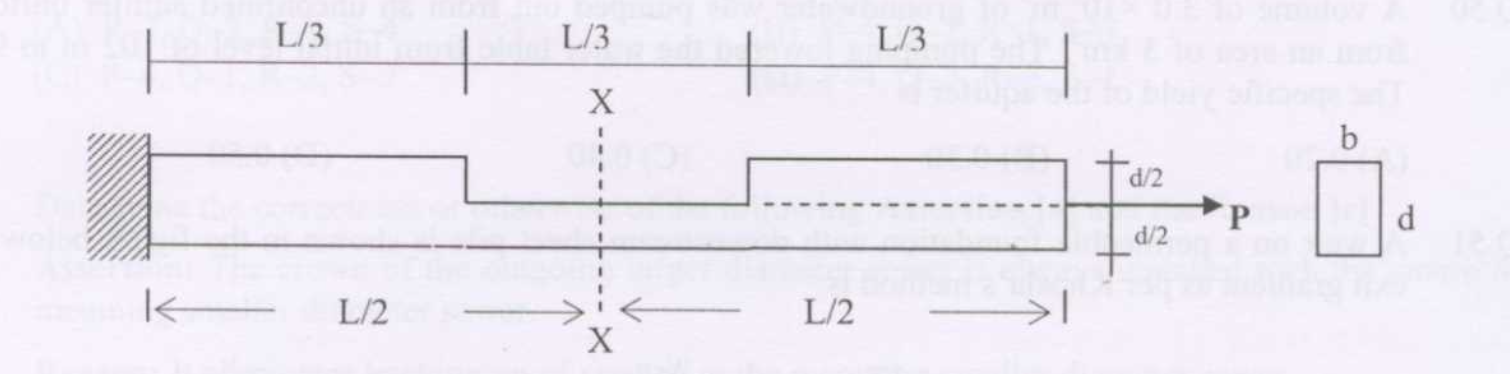
\includegraphics[width=0.6\columnwidth]{figs/fig2.png} 
    \caption{}
    \label{fig:placeholder}
\end{figure}

The critical lane volume on the major road changes to $440$ vehicles per hour per lane and the critical lane volume on the minor road remains unchanged. The green time will


\begin{enumerate}
\item increase for the major road and remain same for the minor road
\item increase for the major road and decrease for the minor road
\item decrease for both the roads
\item remain unchanged for both the roads
\end{enumerate}  


\item It is proposed to widen and strengthen an existing $2$-lane NH section as a divided highway. The existing traffic in one direction is 2500 commercial vehicles \brak{CV} per day. The construction will take $1$ year. The design CBR of soil subgrade is found to be $5$ percent. Given: traffic growth rate for CV = $8$ percent, vehicle damage factor = $3.5$ (standard axles per CV), design life = $10$ years and traffic distribution factor = $0.75$. The cumulative standard axles \brak{msa} computed are \hfill \brak{GATE \ CE \ 2008}
\begin{enumerate}
\begin{multicols}{2}
\item $35$
\item $37$
\item $65$
\item $70$
\end{multicols}
\end{enumerate}

\item A linear relationship is observed between speed and density on a certain section of a highway. The free flow speed is observed to be $80$ km per hour and the jam density is estimated as $100$ vehicles per km length. Based on the above relationship, the maximum flow expected on this section and the speed at the maximum flow will respectively be \hfill \brak{GATE \ CE \ 2008}
\begin{enumerate}
\begin{multicols}{2}
\item $8000$ vehicles per hour and $80$ km per hour
\item $8000$ vehicles per hour and $25$ km per hour
\item $2000$ vehicles per hour and $80$ km per hour
\item $2000$ vehicles per hour and $40$ km per hour
\end{multicols}
\end{enumerate}

\item The plan of a survey plotted to a scale of $10$ m to $1$ cm is reduced in such a way that a line originally $10$ cm long now measures $9$ cm. The area of the reduced plan is measured as $81$ $cm^{2}$?. The actual area $m^{2}$ of the survey is \hfill \brak{GATE \ CE \ 2008}
\begin{enumerate}
\begin{multicols}{2}
\item $10000$
\item $6561$
\item $1000$
\item $656$ 
\end{multicols}
\end{enumerate}

\item The lengths and bearings of a closed traverse PQRSP are given below.



\begin{tabular}{|c|c|c|}
\hline
Line & Length (m) & Bearing (WCB) \\
\hline
PQ & $200$ & $0^\degree$ \\
QR & $1000$ & $45^\degree$ \\
RS & $907$ & $180^\degree$ \\
SP & ? & ? \\
\hline
\end{tabular}



The missing length and bearing, respectively, of the line SP are \hfill \brak{GATE \ CE \ 2008}

\begin{enumerate}
\item $207 m$ and $270^\degree$
\item $707 m$ and $270^\degree$
\item $707 m$ and $180^\degree$
\item $907 m$ and $270^\degree$
\end{enumerate}

\item The focal length of the object glass of a tacheometer is $200$ mm, the distance between the vertical axis of the tacheometer and the optical centre of the object glass is $100$ mm and the spacing between the upper and lower line of the diaphragm axis is $4$ mm. With the line of collimation perfectly horizontal, the staff intercepts are $1$ m \brak{top}, $2$ m \brak{middle}, and $3$ m \brak{bottom}. The horizontal distance \brak{m} between the staff and the instrument station is \hfill \brak{GATE \ CE \ 2008}
\begin{enumerate}
\begin{multicols}{2}
\item $100.3$ 
\item $103.0$ 
\item $150.0$ 
\item $153.0$ 
\end{multicols}
\end{enumerate}

\item A road is provided with a horizontal degreeular curve having deflection angle of $55^\degree$ and centre line radius of $250$ m. A transition curve is to be provided at each end of the circular curve of such a length that the rate of gain of radial acceleration is $0.3$ m/s at a speed of $50$ km per hour. Length of the transition curve required at each of the ends is \hfill \brak{GATE \ CE \ 2008}
\begin{enumerate}
\begin{multicols}{2}
\item $2.57$ 
\item $33.33$ 
\item $35.73$ 
\item $1666.67$ 
\end{multicols}
\end{enumerate}

\item A light house of $120$ m height is just visible above the horizon from a ship. The correct distance \brak{m} between the ship and the light house considering combined correction for curvature and refraction, \hfill \brak{GATE \ CE \ 2008}
\begin{enumerate}
\begin{multicols}{2}
\item $39.098$ 
\item $42.226$ 
\item $39098$ 
\item $42226$ 
\end{multicols}
\end{enumerate}



\textbf{Statement for Linked Answer Questions $71$ and $72$:}


A rectangular channel $6.0$ m wide carries a discharge of $16.0$ m$^3$/s under uniform flow condition with normal depth of $1.60$ m. Manning $n$ is $0.015$. 



\item The longitudinal slope of the channel is \hfill \brak{GATE \ CE \ 2008}

\begin{enumerate}
\item $0.000585$
\item $0.000485$
\item $0.000385$
\item $0.000285$
\end{enumerate}



\item A hump is to be provided on the channel bed. The maximum height of the hump without affecting the upstream flow condition is \hfill \brak{GATE \ CE \ 2008}

\begin{enumerate}
\item $0.50$ m
\item $0.40$ m
\item $0.30$ m
\item $0.20$ m
\end{enumerate}



\item The channel width is to be contracted. The minimum width to which the channel can be contracted without affecting the upstream flow condition is \hfill \brak{GATE \ CE \ 2008}

\begin{enumerate}
\item $3.0$ m
\item $3.8$ m
\item $4.1$ m
\item $4.5$ m
\end{enumerate}



\textbf{Statement for Linked Answer Questions 74 and 75:}

A reinforced concrete beam of rectangular cross section of breadth $230$ mm and effective depth $400 mm$ is subjected to a maximum factored shear force of $120$ $kN$. The grades of concrete, main steel and stirrup steel are $M20$, $Fe415$ and $Fe250$ respectively. For the area of main steel provided, the design shear strength $\tau_c$ as per IS:$456$ --  $2000$ is $0.48$ N/$mm^{2}$. The beam is designed for collapse limit state.



\item The spacing (mm) of 2-legged 8 mm stirrups to be provided is \hfill \brak{GATE \ CE \ 2008}
\begin{enumerate}
\item $40$
\item $115$
\item $250$
\item $400$
\end{enumerate}



\item  In addition, the beam is subjected to a torque whose factored value is $10.90$ kNm. The stirrups have to be provided to carry a shear $kN$ equal to \hfill \brak{GATE \ CE \ 2008}
\begin{enumerate}
\item $50.42$
\item $130.56$
\item $151.67$
\item $200.23$
\end{enumerate}

\section*{Linked Answer Questions: Q.76 to Q.85 carry two marks each}

\textbf{Statement for Linked Answer Questions 76 and 77:}

Beam GHI is supported by three pontoons as shown in the figure below. The horizontal cross-sectional area of each pontoon is $8$ $m^{2}$, the flexural rigidity of the beam is $10000$ kN-$m^{2}$ and the unit weight of water is $10$ kN/$m^{3}$.


\begin{figure}[H]
    \centering
    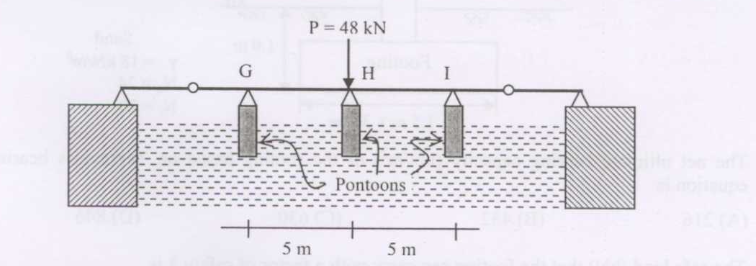
\includegraphics[width=0.6\columnwidth]{figs/fig9.png} 
    \caption{}
    \label{fig:placeholder}
\end{figure}


\item When the middle pontoon is removed, the deflection at H will be \hfill \brak{GATE \ CE \ 2008}
\begin{enumerate}
\item $0.2$ m
\item $0.4$ m
\item $0.6$ m
\item $0.8$ m
\end{enumerate}

\item When the middle pontoon is brought back to its position as shown in the figure above, the reaction at H will be \hfill \brak{GATE \ CE \ 2008}
\begin{enumerate}
\item $8.6$ $kN$
\item $15.7$ $kN$
\item $19.2$ $kN$
\item $24.2$ $kN$
\end{enumerate}


\textbf{Statement for Linked Answer Questions 78 and 79:}

The ground conditions at a site are shown in the figure below.


\begin{figure}[H]
    \centering
    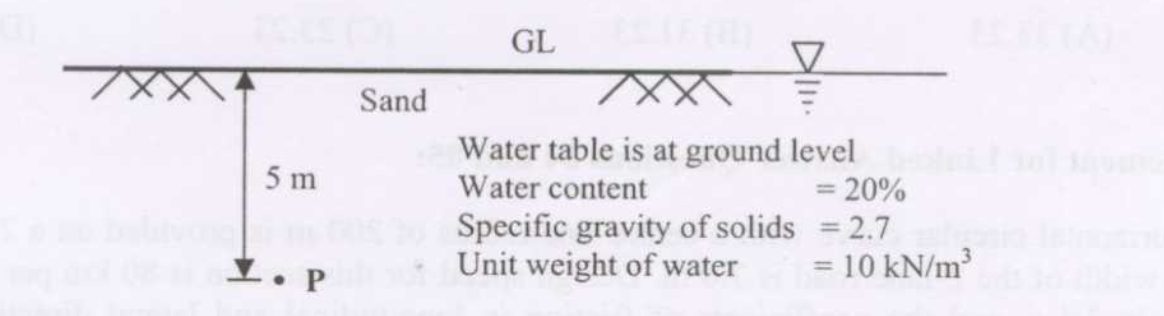
\includegraphics[width=0.6\columnwidth]{figs/fig12.png} 
    \caption{}
    \label{fig:placeholder}
\end{figure}


\item The saturated unit weight of the sand ($kN$/$m^{3}$) is \hfill \brak{GATE \ CE \ 2008}
\begin{enumerate}
\item $15$
\item $18$
\item $21$
\item $24$
\end{enumerate}

\item The total stress, pore water pressure and effective stress (kN/$m^{3}$) at the point P are,  \hfill \brak{GATE \ CE \ 2008}
\begin{enumerate}
\item $75$, $50$ and $25$
\item $90$, $50$ and $40$
\item $105$, $50$ and $55$
\item $120$, $50$ and $70$
\end{enumerate}



\textbf{Statement for Linked Answer Questions 80 and 81:}

A column is supported on a footing as shown in the figure below. The water table is at a depth of $10$ m below the base of the footing.


\begin{figure}[H]
    \centering
    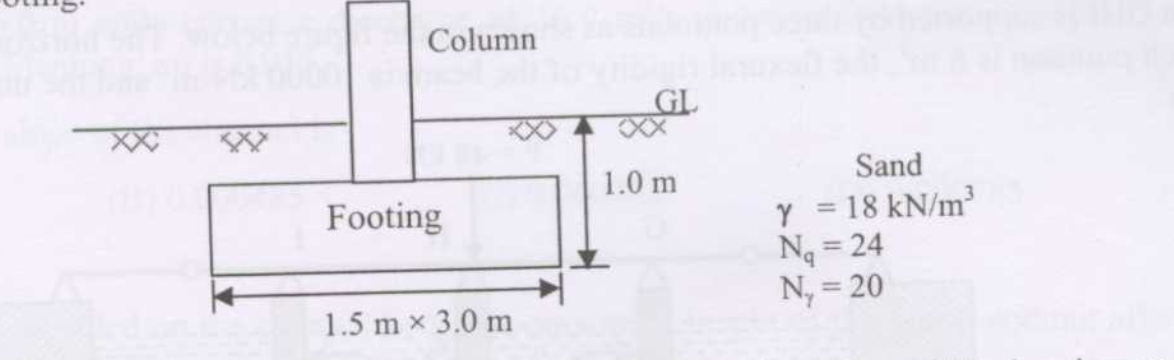
\includegraphics[width=0.6\columnwidth]{figs/fig13.png} 
    \caption{}
    \label{fig:placeholder}
\end{figure}


\item The net ultimate bearing capacity (kN/$m^{2}$) of the footing based on Terzaghi's bearing capacity equation is \hfill \brak{GATE \ CE \ 2008}
\begin{enumerate}
\item $216$
\item $432$
\item $630$
\item $846$
\end{enumerate}

\item The safe load \brak{kN} that the footing can carry with a factor of safety $3$ is \hfill \brak{GATE \ CE \ 2008}
\begin{enumerate}
\item $282$
\item $648$
\item $945$
\item $1269$
\end{enumerate}


\textbf{Statement for Linked Answer Questions 82 and 83:}

An automobile with projected area $2.6$ m\textsuperscript{2} is running on a road with a speed of $120$ km per hour. The mass density and the kinematic viscosity of air are $1.2$ kg/$m^{3}$ and $1.5 \times 10^{-5}$ $m^{2}$/s, respectively. The drag coefficient is $0.30$.

\item The drag force on the automobile is \hfill \brak{GATE \ CE \ 2008}
\begin{enumerate}
\item $620$ N
\item $600$ N
\item $580$ N
\item $520$ N
\end{enumerate}

\item The metric horse power required to overcome the drag force is \hfill \brak{GATE \ CE \ 2008}
\begin{enumerate}
\item $33.23$
\item $31.23$
\item $23.23$
\item $20.23$
\end{enumerate}


\textbf{Statement for Linked Answer Questions 84 and 85:}

A horizontal circular curve with a centre line radius of $200$ m is provided on a $2$-lane, $2$-way SH section. The width of the $2$-lane road is $7.0$ m. Design speed for this section is $80$ km per hour. The brake reaction time is $2.4$ s, and the coefficients of friction in longitudinal and lateral directions are $0.355$ and $0.15$, respectively.


\item The safe stopping sight distance on the section is \hfill \brak{GATE \ CE \ 2008}
\begin{enumerate}
\item $221$ m
\item $195$ m
\item $125$ m
\item $65$ m
\end{enumerate}

\item The set-back distance from the center line of the inner lane is \hfill \brak{GATE \ CE \ 2008}
\begin{enumerate}
\item $7.93$ m
\item $8.10$ m
\item $9.60$ m
\item $9.77$ m
\end{enumerate}


\end{enumerate}
\end{document}